\documentclass{standalone}
\usepackage{tikz}
\usepackage{ctex,siunitx,bm}
\setCJKmainfont{Noto Serif CJK SC}
\usepackage{tkz-euclide,ninecolors}
\usepackage{amsmath}
\usetikzlibrary{patterns, calc}
\usetikzlibrary {decorations.pathmorphing, decorations.pathreplacing, decorations.shapes,}
\begin{document}
\small
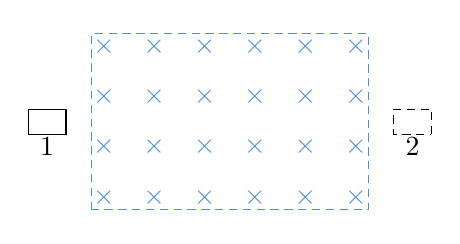
\begin{tikzpicture}[>=latex,scale=0.8]
  \draw[densely dashed,azure6](-2.2,-1.4)rectangle(2.2,1.4);
  \foreach \x in {-2.0,-1.2,-0.4,0.4,1.2,2.0}
  {
    \foreach \y in {-1.2,-0.4,0.4,1.2}
    {
      \node at (\x,\y)[azure6]{$\times$};
    }
  }
  \draw(-3.2,-0.2)rectangle(-2.6,0.2);
  \draw[densely dashed](3.2,-0.2)rectangle(2.6,0.2);
  \node at (-2.9,-0.4){1};
  \node at (2.9,-0.4){2};
\end{tikzpicture}
\end{document}